\documentclass{article}
\usepackage[utf8]{inputenc}
\usepackage[T1]{fontenc}
\usepackage[polish]{babel}
\usepackage{indentfirst}
\usepackage{enumerate}
\usepackage{graphicx}
\usepackage{hyperref}
\usepackage{amsmath}
\usepackage{mathtools}

\title{\huge{\textbf{Platformy programowania (lab10)}}}
\author{Karol Zarębski}
\date{January 2021}

\begin{document}

\begin{titlepage}
\maketitle
\end{titlepage}

\tableofcontents

\newpage
\section{Introduction}
Lorem ipsum dolor sit amet, consectetur adipiscing elit. In eu congue nisi. Aliquam ullamcorper fringilla leo, eu convallis quam pulvinar non. Donec vulputate, massa sed dapibus porttitor, est purus consequat ipsum, in laoreet arcu tortor id erat. Pellentesque ut aliquam tortor.

\subsection{First subsection}
ellentesque ut aliquam tortor. Nullam posuere felis velit, ac maximus ex volutpat vitae. Integer sit amet euismod erat. Aliquam erat volutpat. Morbi ultrices vel urna et dictum. Sed ante neque, mattis at sollicitudin dignissim, convallis accumsan velit. Praesent at lorem ac felis elementum hendrerit id ac mi. Mauris a libero felis.

In hac habitasse platea dictumst. Aenean vel suscipit diam, a ornare metus. Pellentesque eu justo sagittis, blandit nisl et, malesuada odio. Proin et vulputate ligula. Sed eget malesuada sapien. Integer ut gravida nibh. Sed elementum augue mauris, ut varius lectus accumsan at. Nam a lacinia velit. Nulla aliquam auctor feugiat. Praesent eget venenatis orci, vel ultrices mauris.

Pellentesque sagittis tempor cursus. Phasellus nunc purus, bibendum et ex et, posuere imperdiet orci. Nunc posuere efficitur euismod. Nullam placerat, urna sit amet consectetur elementum, ligula erat placerat magna, a vehicula tellus nibh vel purus. Vestibulum at tempus elit, et accumsan lectus. Sed ultricies sem eu nisl accumsan posuere. Aliquam in libero varius lorem tincidunt faucibus. Fusce et fringilla urna, non varius ipsum.

\subsection{Second subsection}
Nulla faucibus lacus id lobortis pretium. Fusce hendrerit tellus ultrices ex consequat, nec consequat diam iaculis. Aenean viverra, ex vel faucibus feugiat, nulla velit placerat arcu, et euismod velit magna tempor elit. Donec quis suscipit ex. Donec convallis vel lectus sed semper. Nunc nec finibus sem, sit amet placerat quam. Morbi lobortis efficitur leo, id finibus purus rutrum id. Quisque in tortor vitae augue dictum pellentesque.

Nullam tempor condimentum tempus. Ut quis tellus sed lacus pellentesque pharetra ac vel enim. In lobortis, augue eu scelerisque euismod, lacus magna gravida ipsum, at blandit ipsum ex fringilla lorem. Nullam gravida accumsan nibh non ullamcorper. Ut auctor justo sed euismod feugiat. Aliquam ac posuere est. Integer posuere in urna sit amet efficitur. Cras imperdiet condimentum ante, faucibus ornare arcu pharetra a. Nulla pharetra ante justo, ut pretium justo pellentesque sed. Mauris metus nisi, lobortis ac mattis quis, auctor sed metus. Phasellus eros sapien, consequat eu convallis fringilla, porta sit amet felis.

Ut congue lacus nec ex accumsan, in ullamcorper lectus feugiat. Mauris at iaculis sem, vel laoreet est. Etiam quam quam, vestibulum quis ligula ut, fringilla lobortis justo. Mauris interdum nunc non tincidunt commodo. Etiam at quam hendrerit, viverra magna vitae, sollicitudin urna. Aenean venenatis, sem ut tincidunt convallis, orci felis mattis justo, eget convallis lectus nibh sit amet ipsum. Aenean eleifend et dui vel vulputate.

Proin auctor metus at elit volutpat, non ultricies dolor varius. Nulla elementum suscipit felis, eu dictum est feugiat a. Vestibulum eu eleifend magna. Sed ut est ut leo pulvinar pharetra nec a dui. Pellentesque porttitor ex sed enim pulvinar consequat. Nunc ac lorem gravida, placerat ex ut, ornare massa. Curabitur interdum sapien vel leo dapibus laoreet. Suspendisse potenti. Donec nisi nulla, pharetra ut cursus non, lobortis et nisi. Mauris faucibus elementum nunc nec molestie. Nunc ut nibh ante. Nunc rutrum, velit vitae congue semper, arcu urna auctor lorem, at volutpat orci sapien vitae sem. Morbi mollis pellentesque felis, et dignissim augue. In blandit rhoncus nibh nec pulvinar. Suspendisse vel est ut lorem varius faucibus in eget erat.

\subsection{Third subsection} \\
\textbf{(textbf)Lorem ipsum dolor sit amet} \\
\texttt{(texttt)Lorem ipsum dolor sit amet} \\
\emph{(emph)Lorem ipsum dolor sit amet}\\
\textit{(textit)Lorem ipsum dolor sit amet} \\
\textsc{(textsc)Lorem ipsum dolor sit amet}\\
\textnormal{(textnormal)Lorem ipsum dolor sit amet}\\

\section{Bibliography references}
\hyperref[sec:bib1]{First bibliography reference}
\newline
\hyperref[sec:bib2]{Second bibliography reference}
\newline
\hyperref[sec:bib3]{Third bibliography reference}
\newline
\hyperref[sec:bib4]{Fourth bibliography reference}

\newpage
\section{List}
\subsection{Number List}

\begin{enumerate}
    \item Grafika i Komunikacja Człowiek - Komputer
    \item Podstawy Ochrony Danych
    \item Platformy Programpowania
    \item Sieci Bezprzewodowe
    \item Systemy Wbudowane
    \item Bazy Danych
\end{enumerate}

\subsection{Point List}

\begin{itemize}
    \item C\#
    \item C++
    \item C
    \item Pyhton
    \item Java
    \item Angular
\end{itemize}

\newpage
\section{Quotation mark}

"Mam 10 pint wody w domu"
\footnote{Pinta - Jednostka miary (1 pinta - 473,176473 mililitra)}
\newline

,,Interesuje się Tanatologią''
\footnote{Tanatologia - Nauka o śmierci człowieka}
\newline

„Zainteresowało mnie słowo Somnambulizm”
\footnote{Somnambulizm - Lunatyzm}

\newpage
\section{Picture and table}
\subsection{Picture}

\label{fig:StarWars}
\begin{figure}[h!]
\centering
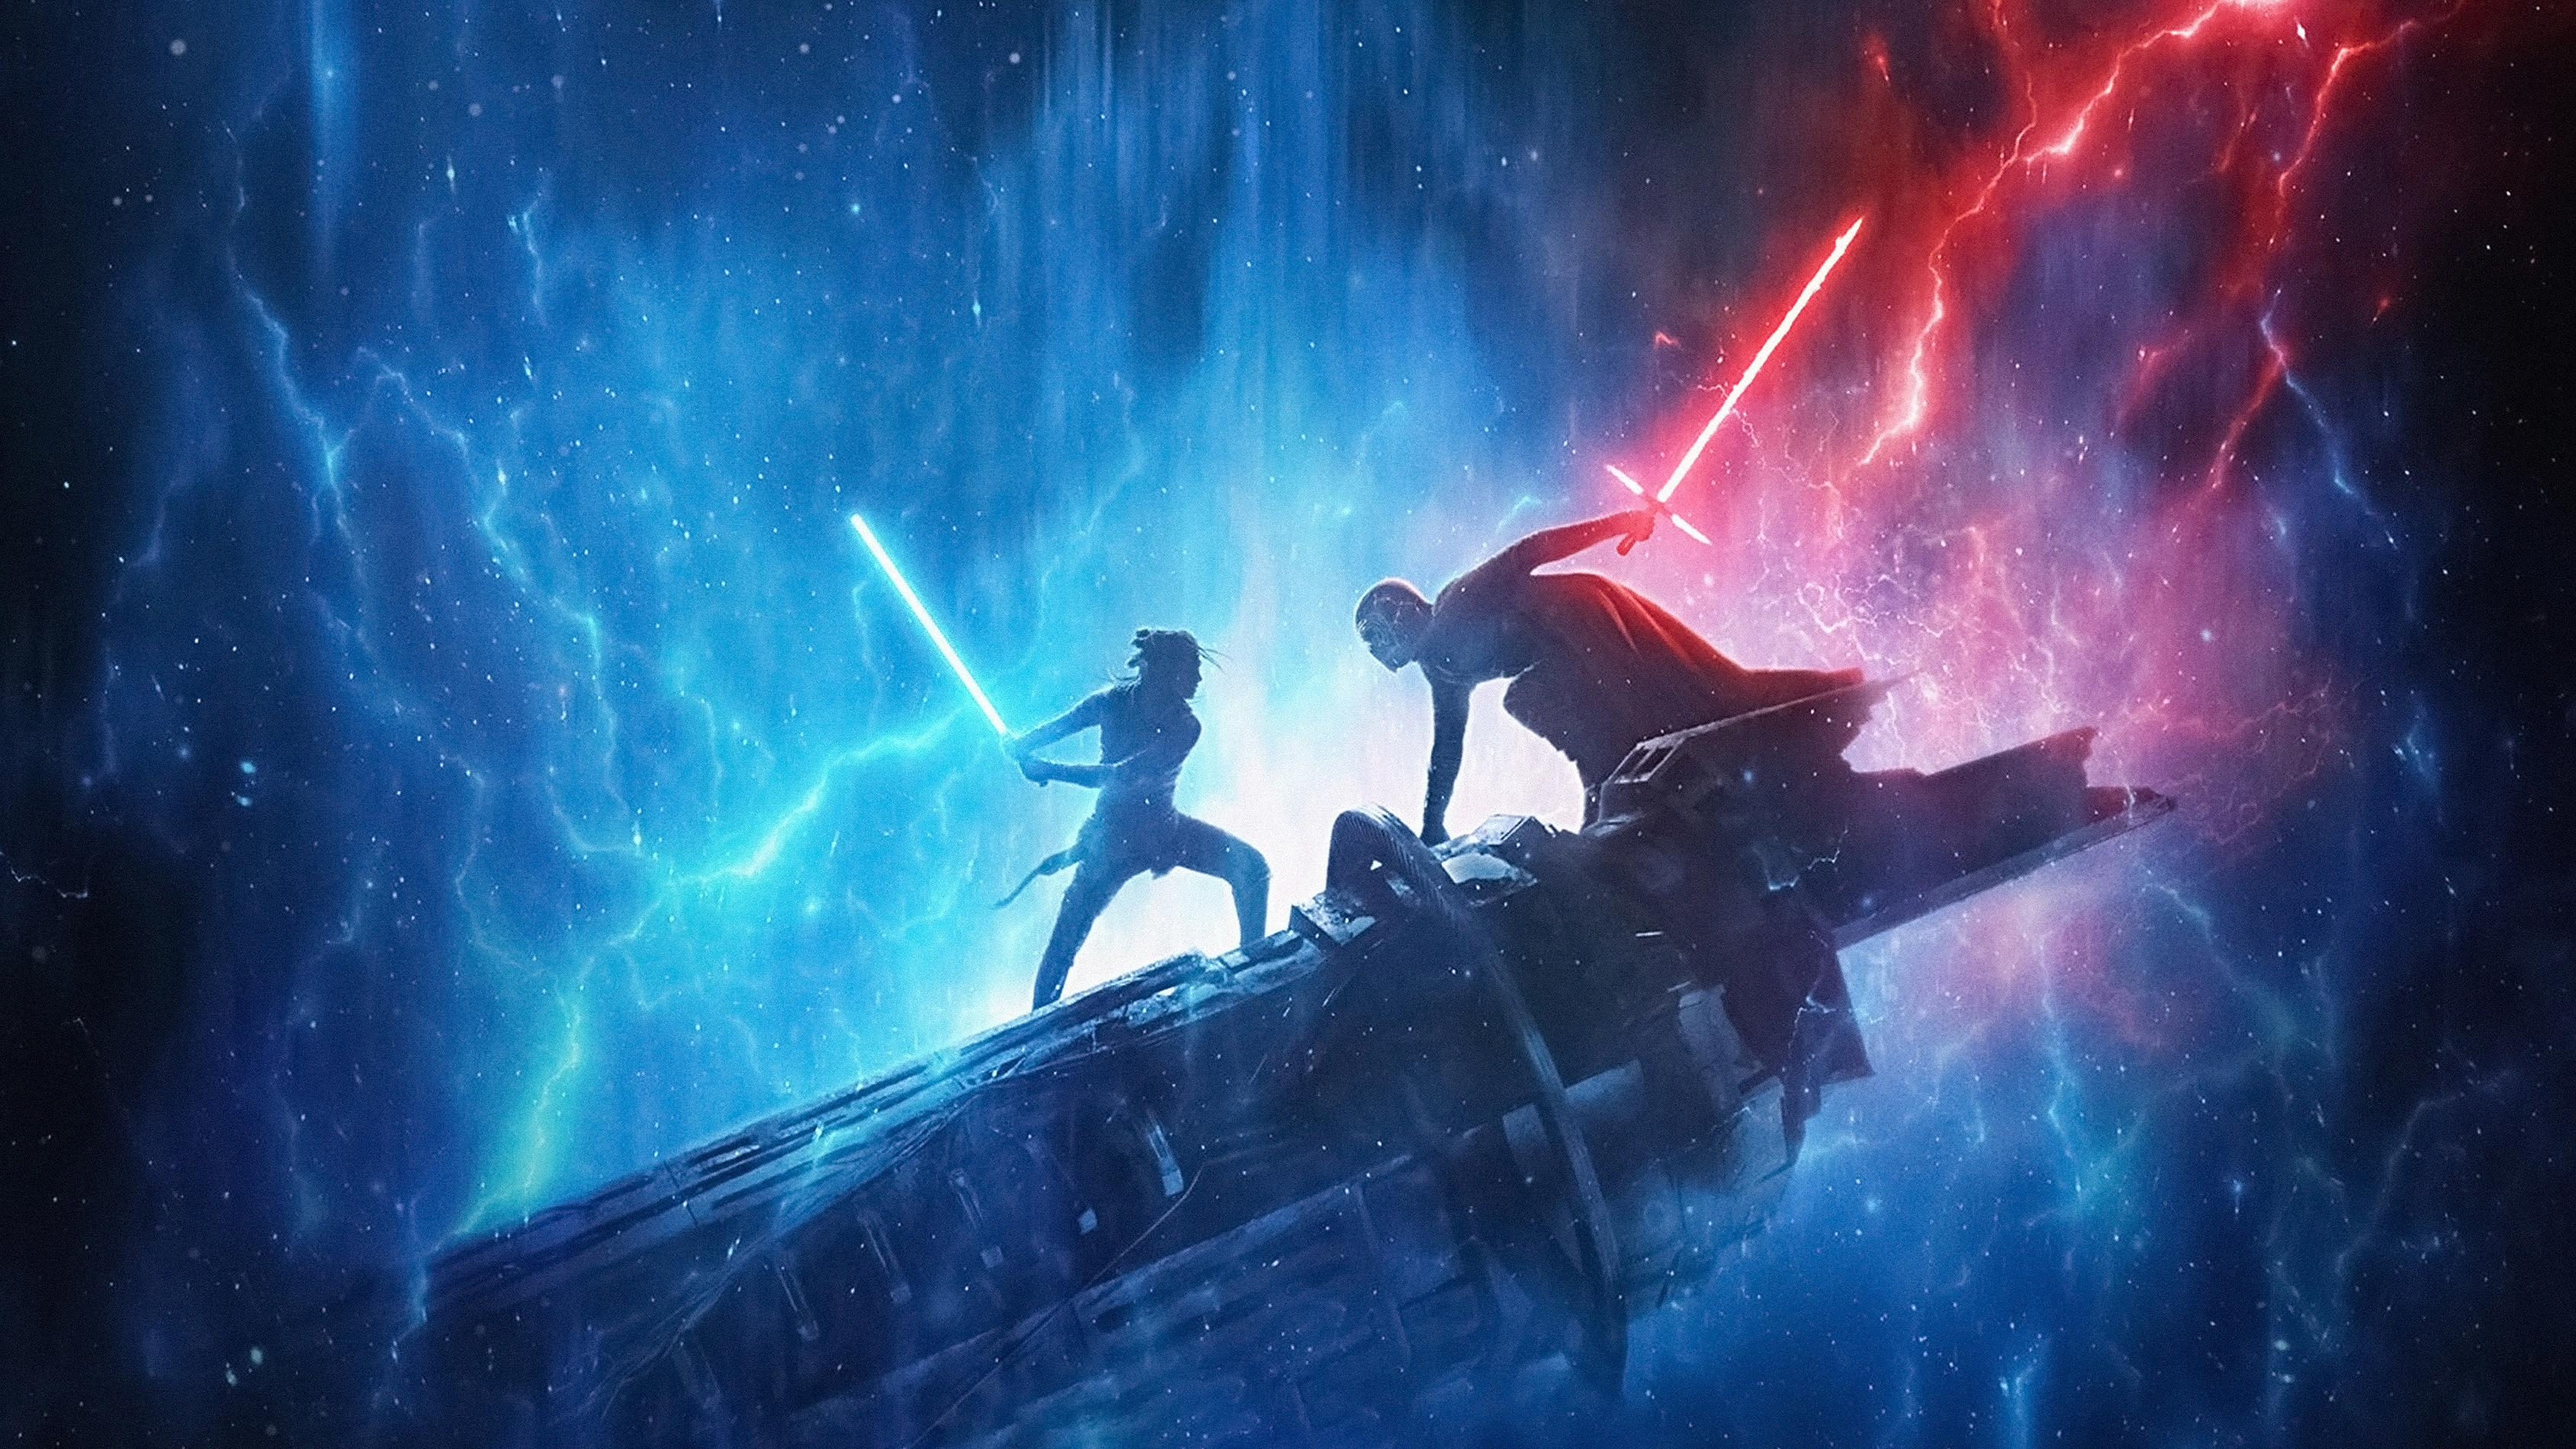
\includegraphics[scale=0.1]{StarWars.jpg}
\caption{The StarWars}
\end{figure}

\subsection{Table}

\label{table:1}
\begin{table}[h!]
\centering
\begin{tabular}{||c c c c||} 
 \hline
 Lp. & Województwo & Powierzchnia[km^{2}] & Populacja \\ [0.5ex] 
 \hline\hline
 1 & Wielkopolskie & 29 826 & 3 475 323 \\ 
 \hline
 2 & Mazowieckie & 35 558 & 5 349 114 \\
 \hline
 3 & Pomorskie & 18 310 & 2 307 710 \\
 \hline
 4 & Małopolskie & 15 183 & 3 372 618 \\
 \hline
 5 & Łódzkie & 18 219 & 2 493 603 \\ [1ex] 
 \hline
\end{tabular}
\caption{Województwa i ich dane}
\end{table}

\subsection{Reference}
\hyperref[fig:StarWars]{Tapeta StarWars}
\newline
\hyperref[table:1]{Tabela województw}
\newline

\newpage
\section{Math}
\begin{enumerate}[a)]
    \item 
        \begin{equation}
            {n \choose k} = \frac{n!}{k!(n - k!)}
        \end{equation}
        
        \item
        \begin{equation}
            a^2 + b^2 = c^2
        \end{equation}
        
        \item
        \begin{equation}
            \frac{\frac{1}{2} + \frac{1}{4}}{\frac{1}{8}}\neq 1
        \end{equation}

        \item
        \begin{equation}
            \sum_{i=1}^{n} i^2 = \frac{n(n + 1)(2n + 1)}{6}
        \end{equation}
        
        \item
        \begin{equation}
            C_2^{-3} + O_2^{0} \rightarrow C^{+4}O_2^{-2} + H_2^{+1}O^{-2}
        \end{equation}
        
        \item
        \begin{equation}
            A_{m,n} = 
            \begin{pmatrix}
                    a_{1,1} & a_{1,2} & \cdots & a_{1,n} \\
                    a_{2,1} & a_{2,2} & \cdots & a_{2,n} \\
                    \vdots & \vdots & \ddots & \vdots \\
                    a_{m,1} & a_{m,2} & \cdots & a_{m,n}
            \end{pmatrix}
        \end{equation}
\end{enumerate}

\newpage
\section{Bibliography}

\begin{thebibliography}{}
\bibitem{Indywidualizm}
\label{sec:bib1}
Daab W.
\textit{Indywidualizm a poglądy społeczno-polityczne, w: Wartości i postawy społeczne a przemiany
systemowe}
 red. J. Reykowski, Warszawa 1993. 
 
 \bibitem{Nowoczesność}
 \label{sec:bib2}
 Giddens A.
 \textit{Nowoczesność i tożsamość}
 Warszawa 2001
 
 \bibitem{Znaczenie}
 \label{sec:bib3}
 Słodczyk R
 \textit{Znaczenie listu w malarstwie XVII i XVIII wieku oraz w ówczesnej powieści epistolarnej}
 „Przestrzenie Teorii” 2009, nr 12, s. 165–191.
 
 \bibitem{Orientacja}
 \label{sec:bib4}
 Zysk T.
 \textit{Orientacja prorozwojowa, w: Orientacje społeczne jako element mentalności}
 red. J. Reykowski,
K. Skarżyńska, M. Ziółkowski, Poznań 1990. 

\end{thebibliography}

\end{document}
